\documentclass[10pt,a4paper]{article}
% common preamble for the WSPR Logger papers
\usepackage[T1]{fontenc}
\usepackage[utf8]{inputenc}
\usepackage{lmodern}
\usepackage{microtype}
\usepackage[a4paper,margin=2.4cm,top=2.6cm,bottom=2.6cm]{geometry}
\usepackage{amsmath}
\usepackage{booktabs}
\usepackage{graphicx}
\usepackage{xcolor}
\usepackage{float}
\usepackage{enumitem}
\usepackage{caption}
\usepackage{fancyhdr}
\usepackage{tabularx}
\usepackage{textcomp}
\usepackage[hidelinks]{hyperref}
\definecolor{accent}{HTML}{2B6CB0}
\captionsetup{font=small,labelfont=bf,labelsep=period,justification=raggedright,singlelinecheck=false}
\setlist{itemsep=2pt,topsep=3pt}
\setlength{\parindent}{0pt}
\setlength{\parskip}{5.5pt plus 1pt}
\renewcommand{\arraystretch}{1.12}
\setcounter{tocdepth}{2}
\pagestyle{fancy}
\fancyhf{}
\renewcommand{\headrulewidth}{0.3pt}
\fancyfoot[C]{\small\thepage}
% Result of `tools/backfill.py --compare 2026-06-01`: six live-logged days rebuilt from wspr.live
\newcommand{\cmpSnaps}{995}
\newcommand{\cmpFrom}{1 June 2026}
\newcommand{\cmpTo}{7 June 2026}
\newcommand{\cmpStored}{41.0}
\newcommand{\cmpRebuilt}{41.0}
\newcommand{\cmpRatio}{1.001}
\newcommand{\cmpMore}{3}
\newcommand{\cmpDxStored}{9.8}
\newcommand{\cmpDxRebuilt}{9.8}
\newcommand{\figwide}[2]{\begin{figure}[htbp]\centering\includegraphics[width=\textwidth]{#1}\caption{#2}\end{figure}}
\newcommand{\figw}[3]{\begin{figure}[htbp]\centering\includegraphics[width=#3\textwidth]{#1}\caption{#2}\end{figure}}
\newcommand{\km}{\,km}
\newcommand{\dB}{\,dB}
\newcommand{\MHz}{\,MHz}
\newcommand{\callsign}[1]{\texttt{#1}}
\newcommand{\keyboxed}[1]{\par\medskip\noindent\fcolorbox{accent}{accent!6}{\begin{minipage}{0.95\textwidth}\small\vspace{3pt}#1\vspace{1pt}\end{minipage}}\par\medskip}
\newcommand{\makeheader}[3]{%
  \begin{center}
    {\Large\bfseries #1\par}\vspace{4pt}
    {\large #2\par}\vspace{8pt}
    {\normalsize Otso Laakso, OH2GAX\par}
    {\small #3\par}
  \end{center}\vspace{2pt}\hrule\vspace{8pt}}

\newcommand{\qcFlagged}{3}
\newcommand{\qcRowsAll}{5\,737}
\newcommand{\qcPairs}{5041}
\newcommand{\qcTol}{500}
\newcommand{\qcCall}{G8LZI/2}
\newcommand{\qcGrid}{JO02gl}
\newcommand{\qcDist}{11\,643}
\newcommand{\qcGridDist}{1\,687}
\newcommand{\qcRows}{3\,483}
\newcommand{\swFrom}{2026-05-08}
\newcommand{\swTo}{2026-11-06}
\newcommand{\swDays}{166}
\newcommand{\swSnap}{18\,885}
\newcommand{\nSeasons}{3}
\newcommand{\nSnap}{54\,868}
\newcommand{\nDays}{495}
\newcommand{\dateFrom}{2024-07-04}
\newcommand{\dateTo}{2026-11-06}
\newcommand{\meanRep}{56.3}
\newcommand{\medRep}{53}
\newcommand{\shareDXsix}{16.3}
\newcommand{\daysDXsix}{360}
\newcommand{\pctDaysDXsix}{73}
\newcommand{\daysDXten}{167}
\newcommand{\pctDaysDXten}{34}
\newcommand{\solarZeroSFI}{76}
\newcommand{\nFofC}{2\,973}
\newcommand{\pctFofC}{16}
\newcommand{\nGaps}{543}
\newcommand{\gapHours}{11528.4}
\newcommand{\nStations}{3\,713}
\newcommand{\nRows}{3\,092\,119}
\newcommand{\nSpots}{42\,723}
\newcommand{\nSpotDays}{490}
\newcommand{\homeShare}{86}
\newcommand{\nTxLoc}{102}
\newcommand{\busyFrom}{7}
\newcommand{\hourMinMed}{2}
\newcommand{\hourMaxMed}{81}
\newcommand{\quietMedMax}{4}
\newcommand{\busyMedAvg}{75}
\newcommand{\qLoMid}{46}
\newcommand{\qHiMid}{99}
\newcommand{\busyTo}{20}
\newcommand{\peakThreeHour}{6}
\newcommand{\peakThreePct}{58}
\newcommand{\lowThreeHour}{13}
\newcommand{\lowThreePct}{22}
\newcommand{\dxPeakHour}{5}
\newcommand{\dxPeakPct}{28}
\newcommand{\dxLowHour}{14}
\newcommand{\dxLowPct}{7}
\newcommand{\dxAtF}{28}
\newcommand{\dxThreeAtF}{46}
\newcommand{\dxAtI}{18}
\newcommand{\dxThreeAtI}{45}
\newcommand{\dxAtBC}{16}
\newcommand{\dxThreeAtBC}{25}
\newcommand{\dxAtBJ}{11}
\newcommand{\dxThreeAtBJ}{54}
\newcommand{\nPairs}{5\,038}
\newcommand{\nBeyondBC}{28}
\newcommand{\nBeyondBCOc}{25}
\newcommand{\nBeyondBCOther}{3}
\newcommand{\qcList}{\callsign{G8LZI\slash 2} (grid JO02gl, listed at 11\,643\km, grid 1\,687\km away); \callsign{SM4HVP} (grid JP70od, listed at 17\,038\km, grid 538\km away); \callsign{SV1CDN} (grid KM17tx, listed at 5\,034\km, grid 2\,535\km away)}
\newcommand{\zneurope}{4207}
\newcommand{\zpeurope}{83.5}
\newcommand{\znnamerica}{120}
\newcommand{\zpnamerica}{2.4}
\newcommand{\znafrica}{60}
\newcommand{\zpafrica}{1.2}
\newcommand{\znpacific}{25}
\newcommand{\zppacific}{0.5}
\newcommand{\znsamerica}{7}
\newcommand{\zpsamerica}{0.1}
\newcommand{\znasia}{9}
\newcommand{\zpasia}{0.2}
\newcommand{\znother}{610}
\newcommand{\zpother}{12.1}
\newcommand{\swPct}{75}
\newcommand{\eastPct}{2}
\newcommand{\northPct}{15}
\newcommand{\secSW}{2865}
\newcommand{\secS}{895}
\newcommand{\secW}{256}
\newcommand{\secSE}{168}
\newcommand{\halfStations}{88}
\newcommand{\topStations}{G4ZFQ, ON5KQ, OE9GHV}
\newcommand{\topStationSnaps}{39\,671}
\newcommand{\snrBandA}{-20}
\newcommand{\snrIqrA}{8}
\newcommand{\snrBandB}{-21}
\newcommand{\snrIqrB}{6}
\newcommand{\snrBandC}{-22}
\newcommand{\snrIqrC}{5}
\newcommand{\snrBandD}{-23}
\newcommand{\snrIqrD}{3}
\newcommand{\snrBandE}{-24}
\newcommand{\snrIqrE}{4}
\newcommand{\snrTopCall}{DK6UG}
\newcommand{\snrTopDB}{+24}
\newcommand{\snrTopDist}{1\,592}
\newcommand{\snrTopDate}{2026-09-17}
\newcommand{\snrLowest}{-35}
\newcommand{\corrDistSNR}{-0.19}
\newcommand{\snrMed}{-21}
\newcommand{\naEarlyH}{5}
\newcommand{\naEarlyPct}{31}
\newcommand{\naDipH}{8}
\newcommand{\naDipPct}{15}
\newcommand{\naLatePct}{9}
\newcommand{\paMornH}{7}
\newcommand{\paMornPct}{11}
\newcommand{\paEveH}{17}
\newcommand{\paEvePct}{12}
\newcommand{\daysNA}{290}
\newcommand{\daysAF}{76}
\newcommand{\daysPA}{161}
\newcommand{\daysSA}{12}
\newcommand{\peaknamerica}{04--07}
\newcommand{\peakpctnamerica}{33}
\newcommand{\peakhnamerica}{10}
\newcommand{\peakafrica}{16--19}
\newcommand{\peakpctafrica}{8}
\newcommand{\peakhafrica}{17}
\newcommand{\peakpacific}{16--19}
\newcommand{\peakpctpacific}{12}
\newcommand{\peakhpacific}{17}
\newcommand{\monBestName}{2026-10}
\newcommand{\monBest}{110}
\newcommand{\monWorstName}{2026-07}
\newcommand{\monWorst}{32}
\newcommand{\monCACEAH}{42}
\newcommand{\monuniqCACEAH}{468}
\newcommand{\monmufCACEAH}{--}
\newcommand{\monsfiCACEAH}{--}
\newcommand{\mondxCACEAH}{9}
\newcommand{\monCACEAI}{62}
\newcommand{\monuniqCACEAI}{660}
\newcommand{\monmufCACEAI}{--}
\newcommand{\monsfiCACEAI}{--}
\newcommand{\mondxCACEAI}{21}
\newcommand{\monCACEAJ}{57}
\newcommand{\monuniqCACEAJ}{457}
\newcommand{\monmufCACEAJ}{--}
\newcommand{\monsfiCACEAJ}{--}
\newcommand{\mondxCACEAJ}{16}
\newcommand{\monCACEBA}{61}
\newcommand{\monuniqCACEBA}{445}
\newcommand{\monmufCACEBA}{--}
\newcommand{\monsfiCACEBA}{--}
\newcommand{\mondxCACEBA}{13}
\newcommand{\monCACFAD}{61}
\newcommand{\monuniqCACFAD}{546}
\newcommand{\monmufCACFAD}{--}
\newcommand{\monsfiCACFAD}{--}
\newcommand{\mondxCACFAD}{5}
\newcommand{\monCACFAE}{65}
\newcommand{\monuniqCACFAE}{707}
\newcommand{\monmufCACFAE}{--}
\newcommand{\monsfiCACFAE}{--}
\newcommand{\mondxCACFAE}{13}
\newcommand{\monCACFAF}{73}
\newcommand{\monuniqCACFAF}{704}
\newcommand{\monmufCACFAF}{--}
\newcommand{\monsfiCACFAF}{--}
\newcommand{\mondxCACFAF}{16}
\newcommand{\monCACFAG}{20}
\newcommand{\monuniqCACFAG}{115}
\newcommand{\monmufCACFAG}{--}
\newcommand{\monsfiCACFAG}{--}
\newcommand{\mondxCACFAG}{0}
\newcommand{\monCACFAI}{82}
\newcommand{\monuniqCACFAI}{755}
\newcommand{\monmufCACFAI}{--}
\newcommand{\monsfiCACFAI}{--}
\newcommand{\mondxCACFAI}{22}
\newcommand{\monCACFAJ}{85}
\newcommand{\monuniqCACFAJ}{798}
\newcommand{\monmufCACFAJ}{--}
\newcommand{\monsfiCACFAJ}{--}
\newcommand{\mondxCACFAJ}{17}
\newcommand{\monCACFBA}{103}
\newcommand{\monuniqCACFBA}{773}
\newcommand{\monmufCACFBA}{--}
\newcommand{\monsfiCACFBA}{--}
\newcommand{\mondxCACFBA}{19}
\newcommand{\monCACFBB}{92}
\newcommand{\monuniqCACFBB}{476}
\newcommand{\monmufCACFBB}{--}
\newcommand{\monsfiCACFBB}{--}
\newcommand{\mondxCACFBB}{1}
\newcommand{\monCACGAD}{96}
\newcommand{\monuniqCACGAD}{661}
\newcommand{\monmufCACGAD}{--}
\newcommand{\monsfiCACGAD}{--}
\newcommand{\mondxCACGAD}{31}
\newcommand{\monCACGAE}{90}
\newcommand{\monuniqCACGAE}{723}
\newcommand{\monmufCACGAE}{--}
\newcommand{\monsfiCACGAE}{--}
\newcommand{\mondxCACGAE}{25}
\newcommand{\monCACGAF}{85}
\newcommand{\monuniqCACGAF}{745}
\newcommand{\monmufCACGAF}{19.8}
\newcommand{\monsfiCACGAF}{121}
\newcommand{\mondxCACGAF}{20}
\newcommand{\monCACGAG}{49}
\newcommand{\monuniqCACGAG}{599}
\newcommand{\monmufCACGAG}{18.8}
\newcommand{\monsfiCACGAG}{139}
\newcommand{\mondxCACGAG}{16}
\newcommand{\monCACGAH}{32}
\newcommand{\monuniqCACGAH}{514}
\newcommand{\monmufCACGAH}{18.1}
\newcommand{\monsfiCACGAH}{133}
\newcommand{\mondxCACGAH}{16}
\newcommand{\monCACGAI}{65}
\newcommand{\monuniqCACGAI}{642}
\newcommand{\monmufCACGAI}{19.9}
\newcommand{\monsfiCACGAI}{117}
\newcommand{\mondxCACGAI}{13}
\newcommand{\monCACGAJ}{99}
\newcommand{\monuniqCACGAJ}{707}
\newcommand{\monmufCACGAJ}{22.5}
\newcommand{\monsfiCACGAJ}{106}
\newcommand{\mondxCACGAJ}{14}
\newcommand{\monCACGBA}{110}
\newcommand{\monuniqCACGBA}{765}
\newcommand{\monmufCACGBA}{24.4}
\newcommand{\monsfiCACGBA}{110}
\newcommand{\mondxCACGBA}{14}
\newcommand{\monCACGBB}{103}
\newcommand{\monuniqCACGBB}{335}
\newcommand{\monmufCACGBB}{26.8}
\newcommand{\monsfiCACGBB}{101}
\newcommand{\mondxCACGBB}{5}
\newcommand{\nFullSw}{6}
\newcommand{\corrMonSFI}{-0.88}
\newcommand{\corrMonMUF}{0.92}
\newcommand{\yrCACEDays}{82}
\newcommand{\yrCACEUniq}{1\,098}
\newcommand{\yrCACEMed}{55}
\newcommand{\yrCACEDx}{15.5}
\newcommand{\yrCACEDxDays}{71}
\newcommand{\yrCACEMax}{15\,619}
\newcommand{\yrCACESnap}{8\,730}
\newcommand{\yrCACFDays}{188}
\newcommand{\yrCACFUniq}{2\,045}
\newcommand{\yrCACFMed}{79}
\newcommand{\yrCACFDx}{14.6}
\newcommand{\yrCACFDxDays}{66}
\newcommand{\yrCACFMax}{15\,619}
\newcommand{\yrCACFSnap}{21\,424}
\newcommand{\yrCACGDays}{225}
\newcommand{\yrCACGUniq}{2\,112}
\newcommand{\yrCACGMed}{82}
\newcommand{\yrCACGDx}{18.1}
\newcommand{\yrCACGDxDays}{79}
\newcommand{\yrCACGMax}{15\,619}
\newcommand{\yrCACGSnap}{24\,714}
\newcommand{\nCommon}{3}
\newcommand{\commonNames}{August, September, October}
\newcommand{\coCACEMed}{60}
\newcommand{\coCACEDx}{17.9}
\newcommand{\coCACEDays}{58}
\newcommand{\coCACFMed}{89}
\newcommand{\coCACFDx}{19.3}
\newcommand{\coCACFDays}{88}
\newcommand{\coCACGMed}{96}
\newcommand{\coCACGDx}{13.6}
\newcommand{\coCACGDays}{82}
\newcommand{\nMonCACE}{4}
\newcommand{\nMonCACF}{7}
\newcommand{\nMonCACG}{8}
\newcommand{\kIdxZero}{113}
\newcommand{\kIdxFive}{88}
\newcommand{\kDxZero}{22}
\newcommand{\kDxOne}{19}
\newcommand{\kDxHi}{7}
\newcommand{\aDxLow}{20}
\newcommand{\aDxHigh}{2.7}
\newcommand{\aIdxHigh}{66}
\newcommand{\aIdxLow}{111}
\newcommand{\mufIdxLow}{27}
\newcommand{\mufIdxMid}{144}
\newcommand{\mufDxLow}{4}
\newcommand{\mufDxMid}{19}
\newcommand{\rMufRaw}{0.70}
\newcommand{\rMufRawLo}{0.67}
\newcommand{\rMufRawHi}{0.74}
\newcommand{\rMufRel}{0.43}
\newcommand{\rMufRelLo}{0.37}
\newcommand{\rMufRelHi}{0.48}
\newcommand{\rSfiRel}{0.05}
\newcommand{\rSfiRelLo}{-0.05}
\newcommand{\rSfiRelHi}{0.15}
\newcommand{\rSfiRaw}{-0.13}
\newcommand{\rKRel}{-0.16}
\newcommand{\rKRelLo}{-0.22}
\newcommand{\rKRelHi}{-0.10}
\newcommand{\caseWorstDay}{2026-07-04}
\newcommand{\caseWorstRep}{10}
\newcommand{\caseJulyK}{7}
\newcommand{\caseJulyA}{74}
\newcommand{\caseJulyRep}{10}
\newcommand{\caseTypRep}{80}
\newcommand{\sfiMax}{203}
\newcommand{\worstAllDay}{2025-03-25}
\newcommand{\worstAllRep}{8}
\newcommand{\worstSwDay}{2026-07-04}
\newcommand{\worstSwRep}{10}
\newcommand{\sfiMin}{89}
\newcommand{\covDays}{381}
\newcommand{\covPct}{77}
\newcommand{\covDaysSw}{131}
\newcommand{\covPctSw}{79}
\newcommand{\recBest}{15\,619}
\newcommand{\recBestCall}{VK7JJ}
\newcommand{\recBestDate}{2024-07-10}
\newcommand{\nOceania}{25}
\newcommand{\cmpDays}{164}
\newcommand{\underDays}{68}
\newcommand{\underPct}{41}
\newcommand{\underExDay}{2026-10-07}
\newcommand{\underExStored}{4\,553}
\newcommand{\underExReplay}{15\,614}

\providecommand{\wFixes}{15\,942}
\providecommand{\wFirst}{2026-05-03}
\providecommand{\wLast}{2026-11-05}
\providecommand{\wSpan}{187}
\providecommand{\wDaysWith}{168}
\providecommand{\wLocs}{72}
\providecommand{\wSqNS}{4.6}
\providecommand{\wSqEW}{4.6}
\providecommand{\wRMS}{1.9}
\providecommand{\wHalfDiag}{3.3}
\providecommand{\wSqArea}{21.3}
\providecommand{\wBits}{24.2}
\providecommand{\wNSq}{18\,662\,400}
\providecommand{\wBitsFour}{15.0}
\providecommand{\wSqFourNS}{111}
\providecommand{\wSqFourEW}{110}
\providecommand{\wMinuteOnly}{2}
\providecommand{\wGapBA}{94}
\providecommand{\wGapDA}{98}
\providecommand{\wGapGA}{99}
\providecommand{\wGapMed}{10}
\providecommand{\wGapGh}{75}
\providecommand{\wPerDayMed}{98}
\providecommand{\wPerDayMax}{143}
\providecommand{\wPerDayMean}{95}
\providecommand{\wHeardPct}{68}
\providecommand{\wTxFrac}{18.4}
\providecommand{\wActiveDays}{164}
\providecommand{\wAvSlotAvg}{67}
\providecommand{\wAvDAAvg}{74}
\providecommand{\wAvGAAvg}{77}
\providecommand{\wAvGAMin}{40}
\providecommand{\wAvGAMinH}{2}
\providecommand{\wAvGAMax}{95}
\providecommand{\wAvDAMin}{34}
\providecommand{\wAvDayDA}{90}
\providecommand{\wAvDayGA}{90}
\providecommand{\wAvNightGA}{46}
\providecommand{\wAvSlotDay}{86}
\providecommand{\wAvSlotNight}{31}
\providecommand{\wRepMed}{14}
\providecommand{\wRepMean}{18.5}
\providecommand{\wRepB}{9}
\providecommand{\wRepD}{85}
\providecommand{\wRepBA}{60}
\providecommand{\wRepDMin}{41}
\providecommand{\wRepDMax}{94}
\providecommand{\wMedHMax}{21}
\providecommand{\wHomePct}{84}
\providecommand{\wNear}{11}
\providecommand{\wMid}{2}
\providecommand{\wFar}{3}
\providecommand{\wFarBAA}{3.1}
\providecommand{\wMaxDist}{193}
\providecommand{\wMaxLoc}{KP31kq}
\providecommand{\wMaxDate}{2026-06-19}
\providecommand{\wKPCAkg}{11}
\providecommand{\wTrips}{5}
\providecommand{\wTripDays}{8}
\providecommand{\wMoves}{296}
\providecommand{\wMoveMed}{4.6}
\providecommand{\wMovePJA}{15}
\providecommand{\wMoveMax}{23}
\providecommand{\wSpeedPJA}{87}
\providecommand{\wChangePct}{2}
\providecommand{\wSteps}{14\,985}
\providecommand{\wHomeWk}{61}
\providecommand{\wHomeWe}{88}
\providecommand{\wNAway}{529}
\providecommand{\wPairDays}{4}
\providecommand{\wRelAway}{153}
\providecommand{\wRelAwayLo}{87}
\providecommand{\wRelAwayHi}{338}
\providecommand{\wRelHome}{100}
\providecommand{\wFloor}{-34}
\providecommand{\wSnrMin}{-35}
\providecommand{\wSnrMax}{24}
\providecommand{\wSnrMed}{-19}
\providecommand{\wSnrQB}{-24}
\providecommand{\wSnrQD}{-14}
\providecommand{\wSnrPF}{-28}
\providecommand{\pwTwoH}{100}
\providecommand{\pwDxTwoH}{100}
\providecommand{\pwRepTwoH}{100}
\providecommand{\pwOneH}{100}
\providecommand{\pwDxOneH}{99}
\providecommand{\pwRepOneH}{99}
\providecommand{\pwFifty}{97}
\providecommand{\pwDxFifty}{93}
\providecommand{\pwRepFifty}{94}
\providecommand{\pwTwentyFive}{88}
\providecommand{\pwDxTwentyFive}{74}
\providecommand{\pwRepTwentyFive}{80}
\providecommand{\pwTen}{72}
\providecommand{\pwDxTen}{46}
\providecommand{\pwRepTen}{57}
\providecommand{\pwFive}{58}
\providecommand{\pwDxFive}{25}
\providecommand{\pwRepFive}{40}
\providecommand{\pwOne}{30}
\providecommand{\pwDxOne}{7}
\providecommand{\pwRepOne}{14}
\providecommand{\wKmW}{78\,095}
\providecommand{\wRecord}{15\,619}
\providecommand{\wAbove}{57}
\providecommand{\wStrongMargin}{15}
\providecommand{\eCapWh}{111}
\providecommand{\eAvgmA}{128}
\providecommand{\eAvgW}{0.64}
\providecommand{\eDays}{6.2}
\providecommand{\eUsable}{94}
\providecommand{\eDaily}{15.3}
\providecommand{\eIdleOnlyDays}{7.9}
\providecommand{\eTxOnlyDays}{3.1}
\providecommand{\eObsLo}{4}
\providecommand{\eObsHi}{5}
\providecommand{\eImpliedLo}{65}
\providecommand{\eImpliedHi}{81}

% Two-page summary of wprs_paper.tex. Every number is a macro written by analyze.py / analyze_wprs.py,
% so this summary stays in step with the full paper when the analysis is re-run.
\newgeometry{margin=1.8cm,top=2.0cm,bottom=1.9cm}
\setlength{\parskip}{4pt plus 1pt}
\captionsetup{font=footnotesize}
\fancyhead[L]{\small WPRS --- two-page summary}
\fancyhead[R]{\small v1.0, 7 November 2026}
\hypersetup{pdftitle={WPRS - Whisper Position Reporting System (two-page summary)},pdfauthor={Otso Laakso, OH2GAX}}
\renewcommand{\makeheader}[3]{%
  \begin{center}
    {\Large\bfseries #1\par}\vspace{2pt}
    {\normalsize #2\par}\vspace{4pt}
    {\small Otso Laakso, OH2GAX \quad---\quad #3\par}
  \end{center}\vspace{0pt}\hrule\vspace{4pt}}
% compact section headings for the summary
\newcommand{\hd}[1]{\par\vspace{5pt}{\large\bfseries\color{accent}#1}\par\vspace{1pt}}
\setlength{\abovecaptionskip}{3pt}\setlength{\belowcaptionskip}{0pt}
\setlength{\textfloatsep}{6pt}\setlength{\intextsep}{6pt}
\begin{document}
\makeheader{WPRS --- Whisper Position Reporting System}{Position beaconing over HF with a 200\,mW WSPR transmitter on a car: a two-page summary}{7 November 2026 --- full paper: \emph{WPRS\_Whisper\_Position\_Reporting\_System.pdf}}

\textbf{The idea.} A WSPR transmitter that computes its Maidenhead locator from a GPS fix turns the worldwide network of volunteer WSPR receivers into a free position channel: no mobile network, no APRS digipeater and no receiver of one's own is needed. Somebody, somewhere, hears the transmission and uploads it to the public WSPR database, and the database is the track. This summary describes the technique and what it achieved from an ordinary car in three summer seasons: \wFixes\ logged transmissions from \wFirst\ to \wLast.

\hd{How it works}
A WSPR transmission lasts 110.6\,s, occupies about 6\,Hz in the 200\,Hz WSPR segment (14\,097.0--14\,097.2\,kHz on 20\,m) and is decoded down to about $-30$\,dB SNR in 2\,500\,Hz. The message carries 50 bits; a \emph{Type~3} message holds a six-character locator, a hash of the callsign and the power. A six-character locator (a \emph{subsquare}, for example KP20jg) is \wSqNS\,$\times$\,\wSqEW\,km at 60\textdegree N, so the position is known with an r.m.s.\ error of \wRMS\,km (at most \wHalfDiag\,km). The four-character locator of an ordinary message would be \wSqFourNS\,km across. A fix reaches the map via the receiver, the WSPR database and \texttt{wspr.live}; the WSPR Logger polls every ten minutes, so a position is visible about 6--10 minutes after it was sent. WPRS is a \emph{breadcrumb trail}, not a live tracker.

\hd{Station}
\textbf{Transmitter:} ZachTek WSPR desktop transmitter, about 200\,mW (23\,dBm), built-in GPS with an external active antenna, one transmission every ten minutes on 20\,m. \textbf{Antenna:} Diamond monoband 14\,MHz whip on a magnetic mount on the roof of a VW Touran (the car body is the ground plane; not fitted in winter, so the data cover March to November). \textbf{Power:} a 30\,000\,mAh USB power bank. At the measured duty cycle (\wTxFrac\,\% transmitting) the average load is \eAvgW\,W and the predicted runtime \eDays\ days; in practice a pack lasts four to five days, and two packs are rotated.

\hd{Results}
\begin{table}[H]\centering\small
\caption{Key measurements, three seasons (2024--2026). A \emph{fix} is a transmission heard by at least one station.}\label{tab:key}
\begin{tabularx}{\textwidth}{@{}lX@{}}\toprule
Data & \wFixes\ fixes on \wDaysWith\ of \wSpan\ days; \wLocs\ different six-character locators; \nStations\ receiving stations \\
Cadence & median \wPerDayMed\ fixes per day (\wHeardPct\,\% of the 144 possible); \wGapBA\,\% of consecutive fixes exactly 10\,min apart \\
Availability & a fix from the previous 60\,min: \wAvDayGA\,\% of the time at 08--16 UTC, \wAvNightGA\,\% at 01--04 UTC (lowest \wAvGAMin\,\% at \wAvGAMinH~UTC) \\
Confirmation & median \wRepMed\ receivers per fix; \wRepD\,\% heard by three or more stations, \wRepB\,\% by a single one \\
Position & home square KP20jg \wHomePct\,\%, adjacent squares \wNear\,\%, more than 25\,km from home \wFar\,\%; farthest fix \wMaxDist\,km (\wMaxLoc, \wMaxDate); \wTrips\ trips beyond 25\,km \\
Coverage & \zpeurope\,\% of the receivers in Europe; a station beyond 6\,000\,km on \pctDaysDXsix\,\% of days; record \wRecord\,km (\wKmW\,km per watt) \\
Lower power & stations still decoding (upper bound): 50\,mW \pwFifty\,\%, 25\,mW \pwTwentyFive\,\%, 10\,mW \pwTen\,\%, 1\,mW \pwOne\,\% \\
Seasons & fixes per median day \sCACEPerDay, \sCACFPerDay, \sCACGPerDay; heard by $\ge$3 stations \sCACERepD, \sCACFRepD, \sCACGRepD\,\% (2024, 2025, 2026) \\\bottomrule
\end{tabularx}\end{table}

\begin{figure}[H]\centering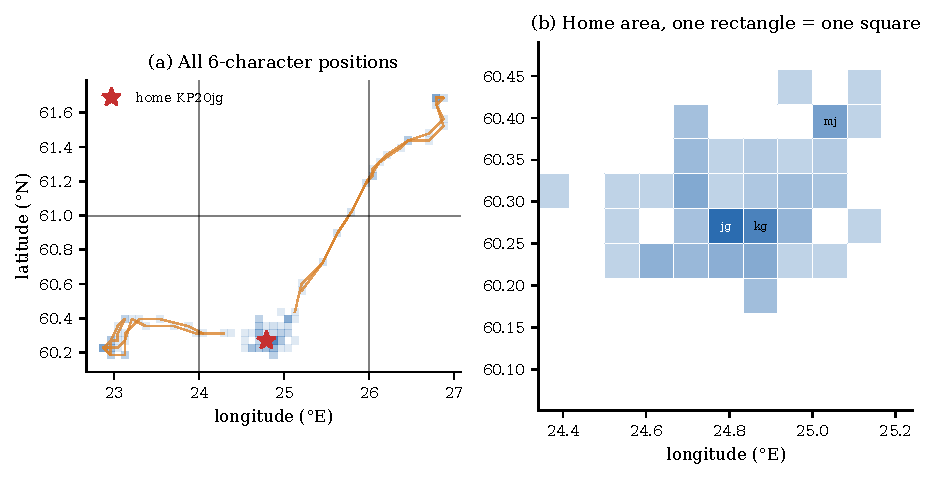
\includegraphics[width=0.74\textwidth]{out/fig_wprs_map.pdf}
\caption{(a) Every six-character position recorded, shaded by number of fixes, with the longest trips. (b) The home area; each rectangle is one subsquare of \wSqNS\,$\times$\,\wSqEW\,km.}\label{fig:map}\end{figure}

\textbf{Availability follows the band.} The transmitter sends every ten minutes; a fix exists when at least one station decodes it. In the daytime the latest position is almost always less than an hour old; in the small hours, when 20\,m is closed, it often is not (Figure~\ref{fig:avail}). Fixes are well confirmed: a typical one is heard by \wRepMed\ independent receivers, which makes a wrong position from a single bad report rare.

\begin{figure}[H]\centering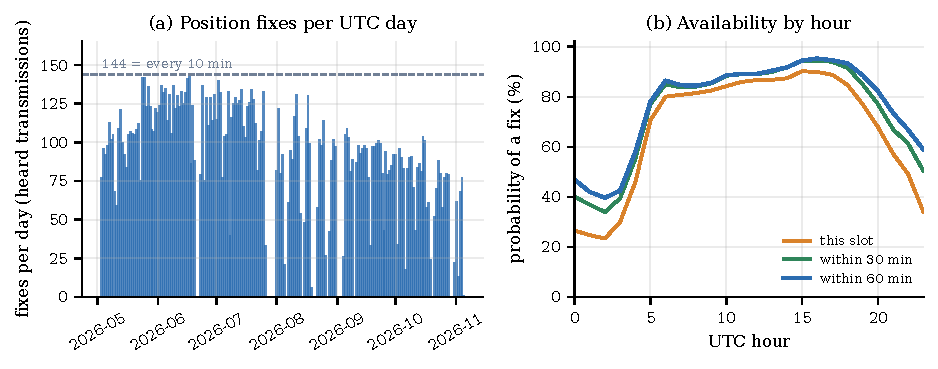
\includegraphics[width=0.95\textwidth]{out/fig_wprs_avail.pdf}
\caption{(a) Position fixes per UTC day over the three seasons. (b) Probability of a fix by UTC hour: from the current slot, from the previous 30 and the previous 60 minutes.}\label{fig:avail}\end{figure}

\textbf{The track is real.} Between 06 and 14 UTC the car is in the home square in \wHomeWk\,\% of the fixes on weekdays but \wHomeWe\,\% at weekends: the commute is recovered from the fixes alone. Trips reached \wMaxDist\,km from home. Two places closer than about five kilometres cannot be told apart; that is the resolution limit of the technique. Most fixes are delivered by European stations one to three thousand kilometres away; the long-distance reports prove the reach but are not needed for tracking. Because European reception is so redundant, even 10\,mW would still have reached \pwTen\,\% of the stations; the long paths would be lost first.

\hd{Where WPRS fits}
Compared with APRS (needs a VHF digipeater or gateway in range) and a cellular GPS tracker (needs mobile coverage and a subscription), WPRS needs no infrastructure and only 0.2\,W, but delivers a square of about 5\,km every ten minutes, with no reverse channel and a gap at night. It suits \emph{away-from-coverage breadcrumb trails} (long drives, hiking, sailing, expeditions) and doubles as a propagation probe. It is not a safety tracker and cannot replace a distress beacon.

\textbf{Limitations.} One car, one antenna and three seasons; the two earlier seasons were rebuilt from \texttt{wspr.live} (checked against a live week: ratio \cmpRatio). No ground-truth GPS log was kept, so the position error is the theoretical one of the locator. A missing fix can mean a closed band, a lost GPS fix, a battery swap or a garage. The track is public: anybody can see where the car is to within about five kilometres, so switch the transmitter off at home if that matters.

\textbf{Operating tips.} Wait for the GPS lock before driving off; give the GPS puck a clear view of the sky; keep the magnetic mount on clean roof metal; do not rely on the latest fix at night; carry a second charged power bank on trips longer than four days.

\keyboxed{\textbf{In short:} a 200\,mW GPS WSPR transmitter with a car-roof whip is a usable infrastructure-free position beacon on 20\,m. It gives a \wSqNS\,km square every ten minutes, a position from the last hour \wAvDayGA\,\% of the daytime and \wAvNightGA\,\% of the night, confirmed by a median of \wRepMed\ receivers, and runs four to five days on a 30\,000\,mAh power bank.}

\end{document}
